\chapter{Teoria de conjuntos}

%Texto baseado em \cite{munkres}.

Habitualmente usaremos letras maiúsculas $A, B, \ldots$ para representar  conjuntos, e letras minúsculas $a, b, \ldots$ para representar seus elementos.
Notações:
\begin{itemize}
 \item Objeto $a$ pertence ao conjunto $A$: $\destaque{a \in A}$.
 \item Objeto $a$ não pertence ao conjunto $A$: $\destaque{a \notin A}$.
 \item Conjunto $A$ está contido no conjunto $B$: $\destaque{A \subset B}$.
 \item Conjunto $A$ contém o conjunto $B$: $\destaque{A \supset B}$.
 \item Conjunto $A$ é subconjunto próprio do conjunto $B$: $\destaque{A \varsubsetneq B}$.
 \item O conjunto que não contém nenhum elemento será denotado por $\destaque{\emptyset}$ = conjunto vazio.
\end{itemize}

\vskip0.4cm

 \begin{exem}
  Sejam $A= \{1, 2, 3, 4, 5 \}$ e $B=\{ 2, 3, 4\}$. Então $1 \in A$, mas $1 \notin B$. Além disso, temos que $B \subset A \Rightarrow A \supset B$.
 \end{exem}

 \vskip0.4cm
 
\section{Operações entre conjuntos}

Dados $A$ e $B$ conjuntos arbitrários dentro do conjunto universo $U$, definimos as seguintes operações entre estes conjuntos:
\begin{itemize}
 \item União: 
 $A \cup B=\{x / x \in A \text{ ou } x \in B\}.$
 
 \begin{venndiagram2sets}
  \fillA \fillB
 \end{venndiagram2sets}

 \vskip0.4cm
 \newpage
 
 \item Interseção: 
 $A \cap B=\{x / x \in A \text{ e } x \in B\}.$
 
 \begin{venndiagram2sets}
  \fillACapB
 \end{venndiagram2sets}
 
 \vskip0.4cm
 
 \item Diferença:
 
 $A - B= \{x | x \in A \text{ e } x \notin B\}.$
 
 \begin{venndiagram2sets}
  \fillANotB
 \end{venndiagram2sets}
 
 $B - A= \{x | x \notin A \text{ e } x \in B\}.$
 
 \begin{venndiagram2sets}
  \fillBNotA
 \end{venndiagram2sets}
 
 \vskip0.4cm
 
 \item Complementares:
 
 $A^{C}= \{x \in U / x \notin A\}$
 
 \begin{venndiagram2sets}
  \fillNotA
 \end{venndiagram2sets}
 
 $B^{C}= \{x \in U / x \notin B\}$
 
 \begin{venndiagram2sets}
  \fillNotB
 \end{venndiagram2sets}
 
 $(A\cap B)^{C}= \{x \in U / x \notin (A\cap B)\}$
 
 \begin{venndiagram2sets}
  \fillNotAorNotB
 \end{venndiagram2sets}
 
 $(A\cup B)^{C}= \{x \in U / x \notin (A\cup B)\}$
 
 \begin{venndiagram2sets}
  \fillNotAorB
 \end{venndiagram2sets}
 
 \vskip0.4cm
 
 \item Produto cartesiano:
 $A \times B= \{(a, b)| a \in A \text{ e } b \in B \}$
 
 O produto cartesiano de dois conjuntos pode ser representado usando eixos coordenados, como mostra o exemplo abaixo. Esta representação é particularmente útil para representar os gráficos de funções de $\R$ para $\R$.
 
 \begin{exem}
  Dados os conjuntos $A= \{1, 2, 3, 4, 5 \}$ e $B=\{ 2, 3, 4, 6\}$, podemos representá-los através do seguinte diagrama de Venn:
  \begin{center}
  \begin{venndiagram2sets}[labelOnlyA={1 5},labelOnlyB={6},labelAB={2  3  4}]
  \end{venndiagram2sets}
  \end{center}
  
  Considerando os conjuntos $A$ e $B$ dados, ao aplicar as operações de conjuntos entre eles obtemos os seguintes conjuntos, e suas respectivas representações através do diagrama de Venn:
  
  \vskip0.4cm
  
  $A \cup B=\{ 1, 2, 3, 4, 5 \}$
  
  \begin{venndiagram2sets}[labelOnlyA={1 5},labelOnlyB={6},labelAB={2  3  4}]
  \fillA \fillB
  \end{venndiagram2sets}
  
  \vskip0.4cm
  
  $A \cap B=\{2, 3, 4 \}$
  
  \begin{venndiagram2sets}[labelOnlyA={1 5},labelOnlyB={6},labelAB={2  3  4}]
  \fillACapB
  \end{venndiagram2sets}
  
  \vskip0.4cm
  
  $A - B= \{1, 5 \}$
  
  \begin{venndiagram2sets}[labelOnlyA={1 5},labelOnlyB={6},labelAB={2  3  4}]
  \fillANotB
  \end{venndiagram2sets}
  
  \vskip0.4cm
  
  \begin{eqnarray*}
   A \times B= \{(1, 2), (1, 3), (1, 4), (1, 6), (2, 2), (2, 3), (2, 4), (2, 6), (3, 2), (3, 3), (3, 4), (3, 6), \\
    (4, 2), (4, 3), (4, 4), (4, 6), (5, 2), (5, 3), (5, 4), (5, 6) \}
  \end{eqnarray*}
  
  \begin{figure}[H]
 \centering
    \fbox{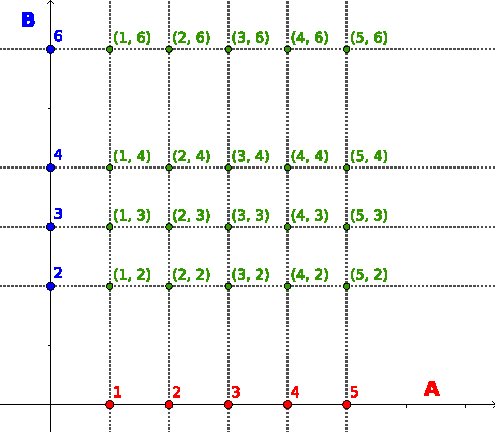
\includegraphics[width=7cm]{../Topicos/Figuras/ProdCartConj.pdf}}
    \caption{Produto cartesiano dos conjuntos $A$ e $B$}
  \end{figure}
  
 \end{exem}
 
 \vskip0.4cm
 
 \newpage
 
 Dada uma família $\mathcal{A}$ de conjuntos, ou seja, dado um conjunto $\mathcal{A}$ de conjuntos, temos:
 \item União de todos os conjuntos que são elementos de $\mathcal{A}$:
 $$\bigcup_{A \in \mathcal{A}} A = \{x| x \in A \text{ para algum } A \in \mathcal{A}\}$$
 \item Interseção de todos os conjuntos que são elementos de $\mathcal{A}$:
 $$\bigcap_{A \in \mathcal{A}} A = \{x| x \in A \text{ para todo } A \in \mathcal{A}\}$$
\end{itemize}

\begin{prop}
Sejam $A$, $B$ e $C$ conjunto arbitrários, temos que:
\begin{itemize}
 \item $\emptyset \subset A$, $\forall A$
 \item $A \cup \emptyset= A$ e $A \cap \emptyset= \emptyset$
 \item $A \cap (B \cup C) = (A \cap B) \cup (A \cap C)$
 \item $A \cup (B \cap C) = (A \cup C) \cap (A \cup C)$
 \item $A - (B \cup C) = (A - B) \cap (A - C)$ (lei de DeMorgan)
 \item $A - (B \cap C) = (A - B) \cup (A - C)$ (lei de DeMorgan)
 \item $\bigcap_{\alpha \in J}(U_{\alpha} \cap Y) = (\bigcap_{\alpha \in J} U_{\alpha}) \cap Y$
 
  $$(U_1 \cap Y) \cap \cdots \cap (U_n \cap Y) = (U_1 \cap \cdots \cap U_n) \cap Y$$
  
 \item $\bigcup_{\alpha \in J}(U_{\alpha} \cap Y) = (\bigcup_{\alpha \in J} U_{\alpha}) \cap Y$
 
 $$(U_1 \cap Y) \cup \cdots \cup (U_n \cap Y) = (U_1 \cup \cdots \cup U_n) \cap Y$$
 
 \item $(U \times V) \cap (A \times B) = (U \cap A) \times (V \cap B)$
 
 \item $X - \bigcap_{\alpha \in J} A_{\alpha} = \bigcup_{\alpha \in J}(X - A_{\alpha})$
 
 \item $X - \bigcup_{i= 1}^{n} A_i = \bigcap_{i = 1}^{n}(X - A_i)$
 
\end{itemize}
\end{prop}

 A \textbf{cardinalidade} de um conjunto $A$ qualquer, é o número de elementos deste conjunto. Denotada por: $|A|$ ou $\# A$. 
 
 Note que: $\# \emptyset= 0$.
 
 Dados dois conjuntos $A$ e $B$ quaisquer é importante observar que:
 \vskip0.3cm
 \colorbox{azul}{
 \begin{minipage}{14.5cm}
 \begin{center}
 a cardinalidade da união destes dois conjuntos é dada por:
  \[\#(A \cup B)= \# A + \# B - \#(A \cap B) \ .\]
 \end{center}
 \end{minipage}}
 \vskip0.3cm
 
 Esta fórmula irá nos ajudar a resolver muitos problemas de teoria de conjuntos.

\newpage

\section{Exercícios - Nível Fácil}
\begin{enumerate}
 \item Considerando os conjuntos $A= \{0,1,2,3\}$,  $B=\{0,2,4,6,8\}$, $C= \{1,3,5,7,9\}$ use os símbolos $\in$, $\notin$ para relacionar:
 \begin{multicols}{4}
  $0 \underline{\hspace{1cm}} A$; \\ $5 \underline{\hspace{1cm}} A$; \\ $6 \underline{\hspace{1cm}} A$; \\ $7 \underline{\hspace{1cm}} A$;\\
  $0 \underline{\hspace{1cm}} B$; \\ $9 \underline{\hspace{1cm}} B$; \\ $8 \underline{\hspace{1cm}} B$; \\ $1 \underline{\hspace{1cm}} B$;\\
  $2 \underline{\hspace{1cm}} C$; \\ $5 \underline{\hspace{1cm}} C$; \\ $8 \underline{\hspace{1cm}} C$; \\ $3 \underline{\hspace{1cm}} C$.
 \end{multicols}

 
 
 \item Considerando os conjuntos $A= \{0,1,2,3\}$,  $B=\{0,1,2,3,4,5\}$, $C= \{3,4,5,6\}$ use os símbolos $\subset$, $\nsubseteq$ para relacionar:
 \begin{multicols}{3}
  $A \underline{\hspace{1cm}} B$; \\ $A \underline{\hspace{1cm}} C$; \\ $B \underline{\hspace{1cm}} C$; \\ 
  $B \underline{\hspace{1cm}} A$; \\ $C \underline{\hspace{1cm}} A$; \\ $C \underline{\hspace{1cm}} B$; \\
  $\emptyset \underline{\hspace{1cm}} A$; \\ $\emptyset \underline{\hspace{1cm}} B$; \\ $\emptyset \underline{\hspace{1cm}} C$.
 \end{multicols}
 
  \item Considerando os conjuntos $A= \{0,1,2,3\}$,  $B=\{0,1,2,3,4,5\}$, $C= \{3,4,5,6\}$ use os símbolos        $\supset$, $\nsupseteq$ para relacionar:
 \begin{multicols}{3}
  $A \underline{\hspace{1cm}} B$; \\ $A \underline{\hspace{1cm}} C$; \\ $B \underline{\hspace{1cm}} C$; \\ 
  $B \underline{\hspace{1cm}} A$; \\ $C \underline{\hspace{1cm}} A$; \\ $C \underline{\hspace{1cm}} B$; \\
  $\emptyset \underline{\hspace{1cm}} A$; \\ $\emptyset \underline{\hspace{1cm}} B$; \\ $\emptyset \underline{\hspace{1cm}} C$.
 \end{multicols}
 
 \item Determine $x$ para que $\{5,6,7,7,8\}= \{5,x,7,8\}$.
 \vskip0.5cm
 
 \item Determine $a$ para que $\{a,2,6\} \subset \{1,2,2,6,10\}$.
 \vskip0.5cm
 
 \item Dados os conjuntos $A=\{a, b, c, e, i, o, u\}$ e $B=\{a, e, i, o, u\}$. Classifique como verdadeiro (V) ou falso (F):
 \begin{multicols}{2}
 \begin{enumerate}[a)]
 \item $(\hspace{0.4cm})$ $B \subset A$.
 \item $(\hspace{0.4cm})$ $A-B= \{a, b, c\}$.
 \item $(\hspace{0.4cm})$ $B \supset A$.
 \item $(\hspace{0.4cm})$ $B-A= \emptyset$.
 \item $(\hspace{0.4cm})$ $\emptyset \subset A$.
 \item $(\hspace{0.4cm})$ $\emptyset \in B$.
 \end{enumerate}
 \end{multicols}
 
 \item Considerando os conjuntos $A=\{a, b, c, e, i, o, u\}$, $B=\{a, e, i, o, u\}$, $C=\{a,b,c,d,e\}$. Relacione as duas colunas:
 \begin{multicols}{2}
   \begin{enumerate}[a)]
 \item $B \cup A$.
 \item $A-B$.
 \item $C \cap B$.
 \item $A \cup C$.
 \item $B - C $.
 \item $A \cap B $.
 \end{enumerate}
 
  $(\hspace{0.4cm})$ $\{a,e\}$.\\
  $(\hspace{0.4cm})$ $B$.\\
  $(\hspace{0.4cm})$ $A$.\\
  $(\hspace{0.4cm})$ $\{a,b,c,d,e,i,o,u\}$.\\
  $(\hspace{0.4cm})$ $\{b, c\}$.\\
  $(\hspace{0.4cm})$ $\{i,o,u\}$.
 
 \end{multicols}


\end{enumerate}

\newpage
\section{Exercícios - Nível Médio}

\begin{enumerate}
 \item Escreva o conjunto expresso pela propriedade:
 \begin{enumerate}[a)]
  \item A é o conjunto dos números pares maiores que 12 e menores que 23.
   \vskip0.5cm
   
  \item B é o conjunto dos múltiplos de 5 menores que 30.
   \vskip0.5cm
   
  \item C é o conjunto dos divisores de 15.
   \vskip0.5cm
   
  \item D é o conjunto dos números ímpares maiores ou iguais a 7 e menores que 26.
   \vskip0.5cm
 \end{enumerate}
 
 \item Escreva uma propriedade que define o conjunto:
 \begin{enumerate}[a)]
  \item $A=\{0, 1, 2, 3, 4, 5, 6, 7, 8, 9\}$
   \vskip0.5cm
  \item $B=\{11, 13, 15, 17\}$
   \vskip0.5cm
  \item $C=\{0,3,6,9,12, \cdots \}$
 \end{enumerate}
 
 \item Classifique os conjuntos abaixo em vazio, unitário, finito ou infinito:
 \begin{enumerate}[a)]
  \item $A$ é o conjunto das soluções da equação $2x+5=19$.
   \vskip0.5cm
  \item $B = \{x \mid x \text{ é um número natural maior que 10 e menor que 11}\}$.
   \vskip0.5cm
  \item $C = \{2,5,8,11, \cdots \}$
   \vskip0.5cm
  \item $D= \{7, 14, 21, 28, \cdots, 70\}$
   \vskip0.5cm
  \item $E= \{2,4,8,16,32,64, \cdots \}$
   \vskip0.5cm
 \end{enumerate}
 
 \item Em uma escola, 100 alunos praticam basquete, 150 praticam futebol, 20 alunos praticam basquete e futebol e 110 alunos não praticam esportes. Qual o número total de alunos da escola?
 
 
 \item Em um concurso foram entrevistados 979 candidatos, dos quais 527 falam a língua inglesa, 251 a língua espanhola e 321 não falam nenhum desses idiomas. O número de candidatos que falam as línguas inglesa e espanhola é? 




  \item (IESES - 2017)  Sabendo que temos os conjuntos $A$ e $B$ é \textbf{INCORRETO} afirmar sobre a teoria dos conjuntos que:
  \begin{enumerate}[a)]
  \item A e B são disjuntos quando não possuírem intersecção.
  \item União de A com B é o conjunto formado por elementos que pertencem a A ou B.
  \item Se B é um subconjunto de A, a complementar de A em B é igual a B – A.
  \item Intersecção de A com B é o conjunto dos elementos em comum a A e B.
  \end{enumerate}
  
  \item (CESGRANRIO-2012) Se $P$, $M$ e $N$ são conjuntos e $x$ é tal que $x \notin P \cup M \cup N$ , então:
  \begin{enumerate}[a)]
  \item $x \notin P$  e $x  \notin M$  e $x \notin N$;
  \item $x \notin P$ ou $x \notin M$ ou $x \notin N$;
  \item $x \notin P$ ou $x \notin M \cup N$;
  \item $x \notin P \cap M$ e $x \notin N$;
  \item $x \notin P \cup M$ ou $x \notin N$.
  \end{enumerate}
  
  \item (Quadrix - 2014)  Considere os conjuntos: 
      \[F = \{2, 5, 6, 9,10 \}\]
      \[G = \{3, 4, 7, 8, 12\}\]
 Sabe-se que o conjunto $H$ é formado por uma operação realizada entre os conjuntos $F$ e $G$. Assinale a alternativa que  contém a operação realizada entre os conjuntos $F$ e $G$, que tem como resultado o conjunto $H$, sendo que $H = \varnothing$.
 \begin{enumerate}[a)]
  \item $H= (F \cup G)$;
  \item $H= (F \cap G)$;
  \item $H= (F - G)$;
  \item $H= (G - F)$;
  \item $H= (G \cup F)$.
 \end{enumerate}
  
  \end{enumerate}
  
\newpage
\section{Exercícios - Nível Difícil}

 \begin{enumerate}
  \item (FGV - 2017) Manoel cria coelhos e seus animais ou são brancos ou são marrons. Do total dos 120 coelhos que possui, 63 são fêmeas, 50 são marrons e, dos machos, 32 são brancos. O número de fêmeas marrons é:
  \begin{enumerate}[a)]
  \item 25;
  \item 27;
  \item 29;
  \item 31;
  \item 33.
  \end{enumerate}
  
   \item (SOCIESC - Téc. Enfermagem) Dentre as várias opções para compor o prato de almoço do restaurante do Arnaldo, está o feijão e o arroz. De todas as 328 pessoas que almoçaram lá, num determinado período, apenas 20 não optaram por, pelo menos, um dos ingredientes, contra a grande maioria que optou ou em comer somente o arroz, somente o feijão ou, ainda, em misturá-los. Assinale a alternativa que descreve a quantidade total de pessoas que optaram em comer feijão com arroz, se o total de pessoas que NÃO comeram arroz é de 100 pessoas e sabendo que 110 pessoas NÃO comeram feijão.
  \begin{enumerate}
  \item 90
  \item 80
  \item 218
  \item 228
  \item 138
 \end{enumerate}
 
  \item (Lógica - Fundatec - 2018) Em um condomínio de 245 condôminos, sabe-se que 125 usam o salão de jogos, 96 usam o salão de jogos e a piscina. Mas 74 não usam o salão de jogos nem a piscina. Quantos condôminos usam a piscina e não usam o salão de jogos?
  \begin{enumerate}[a)]
  \item 29
  \item 46
  \item 75
  \item 120
  \item 149
  \end{enumerate}

  
  \end{enumerate}
 

% \begin{enumerate}[a)]
%  \item 
%  \end{enumerate}
 




